\chapter{Approaching Word2Vec-$\theta$RARes Language Model} \label{approach}

So far we have seen the basics of Word2Vec model and the Echo State Network. We have also seen the functioning and possible limitation of the $\theta$RARes model. In this chapter, we will see the models proposed to validate the research hypothesis formulated in the previous chapter.  First the Word2Vec-$\theta$RARes neural language model in an extension to the $\theta$RARes model will be described, and then the Word2Vec-ESN classifier that could also be used for the TRA task will be discussed.

\section{Word2Vec-$\theta$RARes Language Model} \label{sec:w2v-esn_model}

This research proposes a Word2Vec-$\theta$RARes language model for the TRA task. The proposed model is inspired from the $\theta$RARes model proposed by Hinaut et al. \cite{xavier:2013:RT} for TRA task. Figure \ref{fig:model_arch} shows the basic architecture of Word2Vec-$\theta$RARes model. The Word2Vec-$\theta$RARes model is a combination of Word2Vec model and Echo State Network (ESN). The Word2Vec model is responsible for generating the distributed embeddings of the words in the input sentences. The generated word embeddings are then input to ESN which further processes these word embeddings to learn and predict the thematic roles of all semantic words in the input sentences.

\begin{figure}[hbtp]
\centering

\includegraphics[width=0.9\linewidth]{model_arch}
\caption[Architecture of Word2Vec-$\theta$RARes model.]{\textbf{Architecture of Word2Vec-$\theta$RARes model:} { \small The model takes the words of a sentence as an input across time. Word2Vec model generates the distributed vector representation of the input words. ESN then uses the generated word vectors for further processing to learn and predict the coded meaning of an input sentence.}}
\label{fig:model_arch}
\end{figure}

\paragraph{Model initialization:}Before using the Word2Vec-$\theta$RARes model for the TRA task, the Word2Vec model is trained using the skip-gram negative sampling \cite{w2v:mikolov_2013_distributed} on a general purpose dataset (e.g. Wikipedia) and the domain specific dataset. During the training of Word2Vec model, the low dimensional distributed embeddings for each word in the corpus vocabulary is learned.

To initialize the ESN, firstly, a reservoir of size $N_{x}$ composed of leaky integrator neurons and \textit{tanh} activation function is created. The input-to-hidden weights ($W^{in}$) and hidden to hidden weights ($W^{res}$) are then generated sparsely and randomly from a Gaussian distribution with mean 0 and variance 1. These weights once initialized are fixed and remains unchanged during the training \cite{esn:scholarpedia:2007, esn:practical_guide}. To generate the weights sparsely, a fixed fan-out of $F_{hh}$ and $F_{ih}$ is chosen for hidden-to-hidden and input-to-hidden connections respectively. In other words, each reservoir neuron is connected randomly to $F_{hh}$ other reservoir neurons and each input neurons are connected randomly to only $F_{ih}$ reservoir neurons. 

\subsection{Training Word2Vec-$\theta$RARes model}

The Word2Vec-$\theta$RARes language model treats the TRA task as a prediction problem. The objective of this model is to learn and predict the thematic roles of all semantic words in the input sentence. To evaluate the performance of this model, meaning error and sentence error metrics are used (see section \ref{sec:evaluation_metrics_1}). The same evaluation metrics were used to evaluate $\theta$RARes model \cite{xavier:2013:RT}. Thus it enables us to compare the performance of both Word2Vec-$\theta$RARes and $\theta$RARes model.


\begin{figure}[hbtp]
\centering
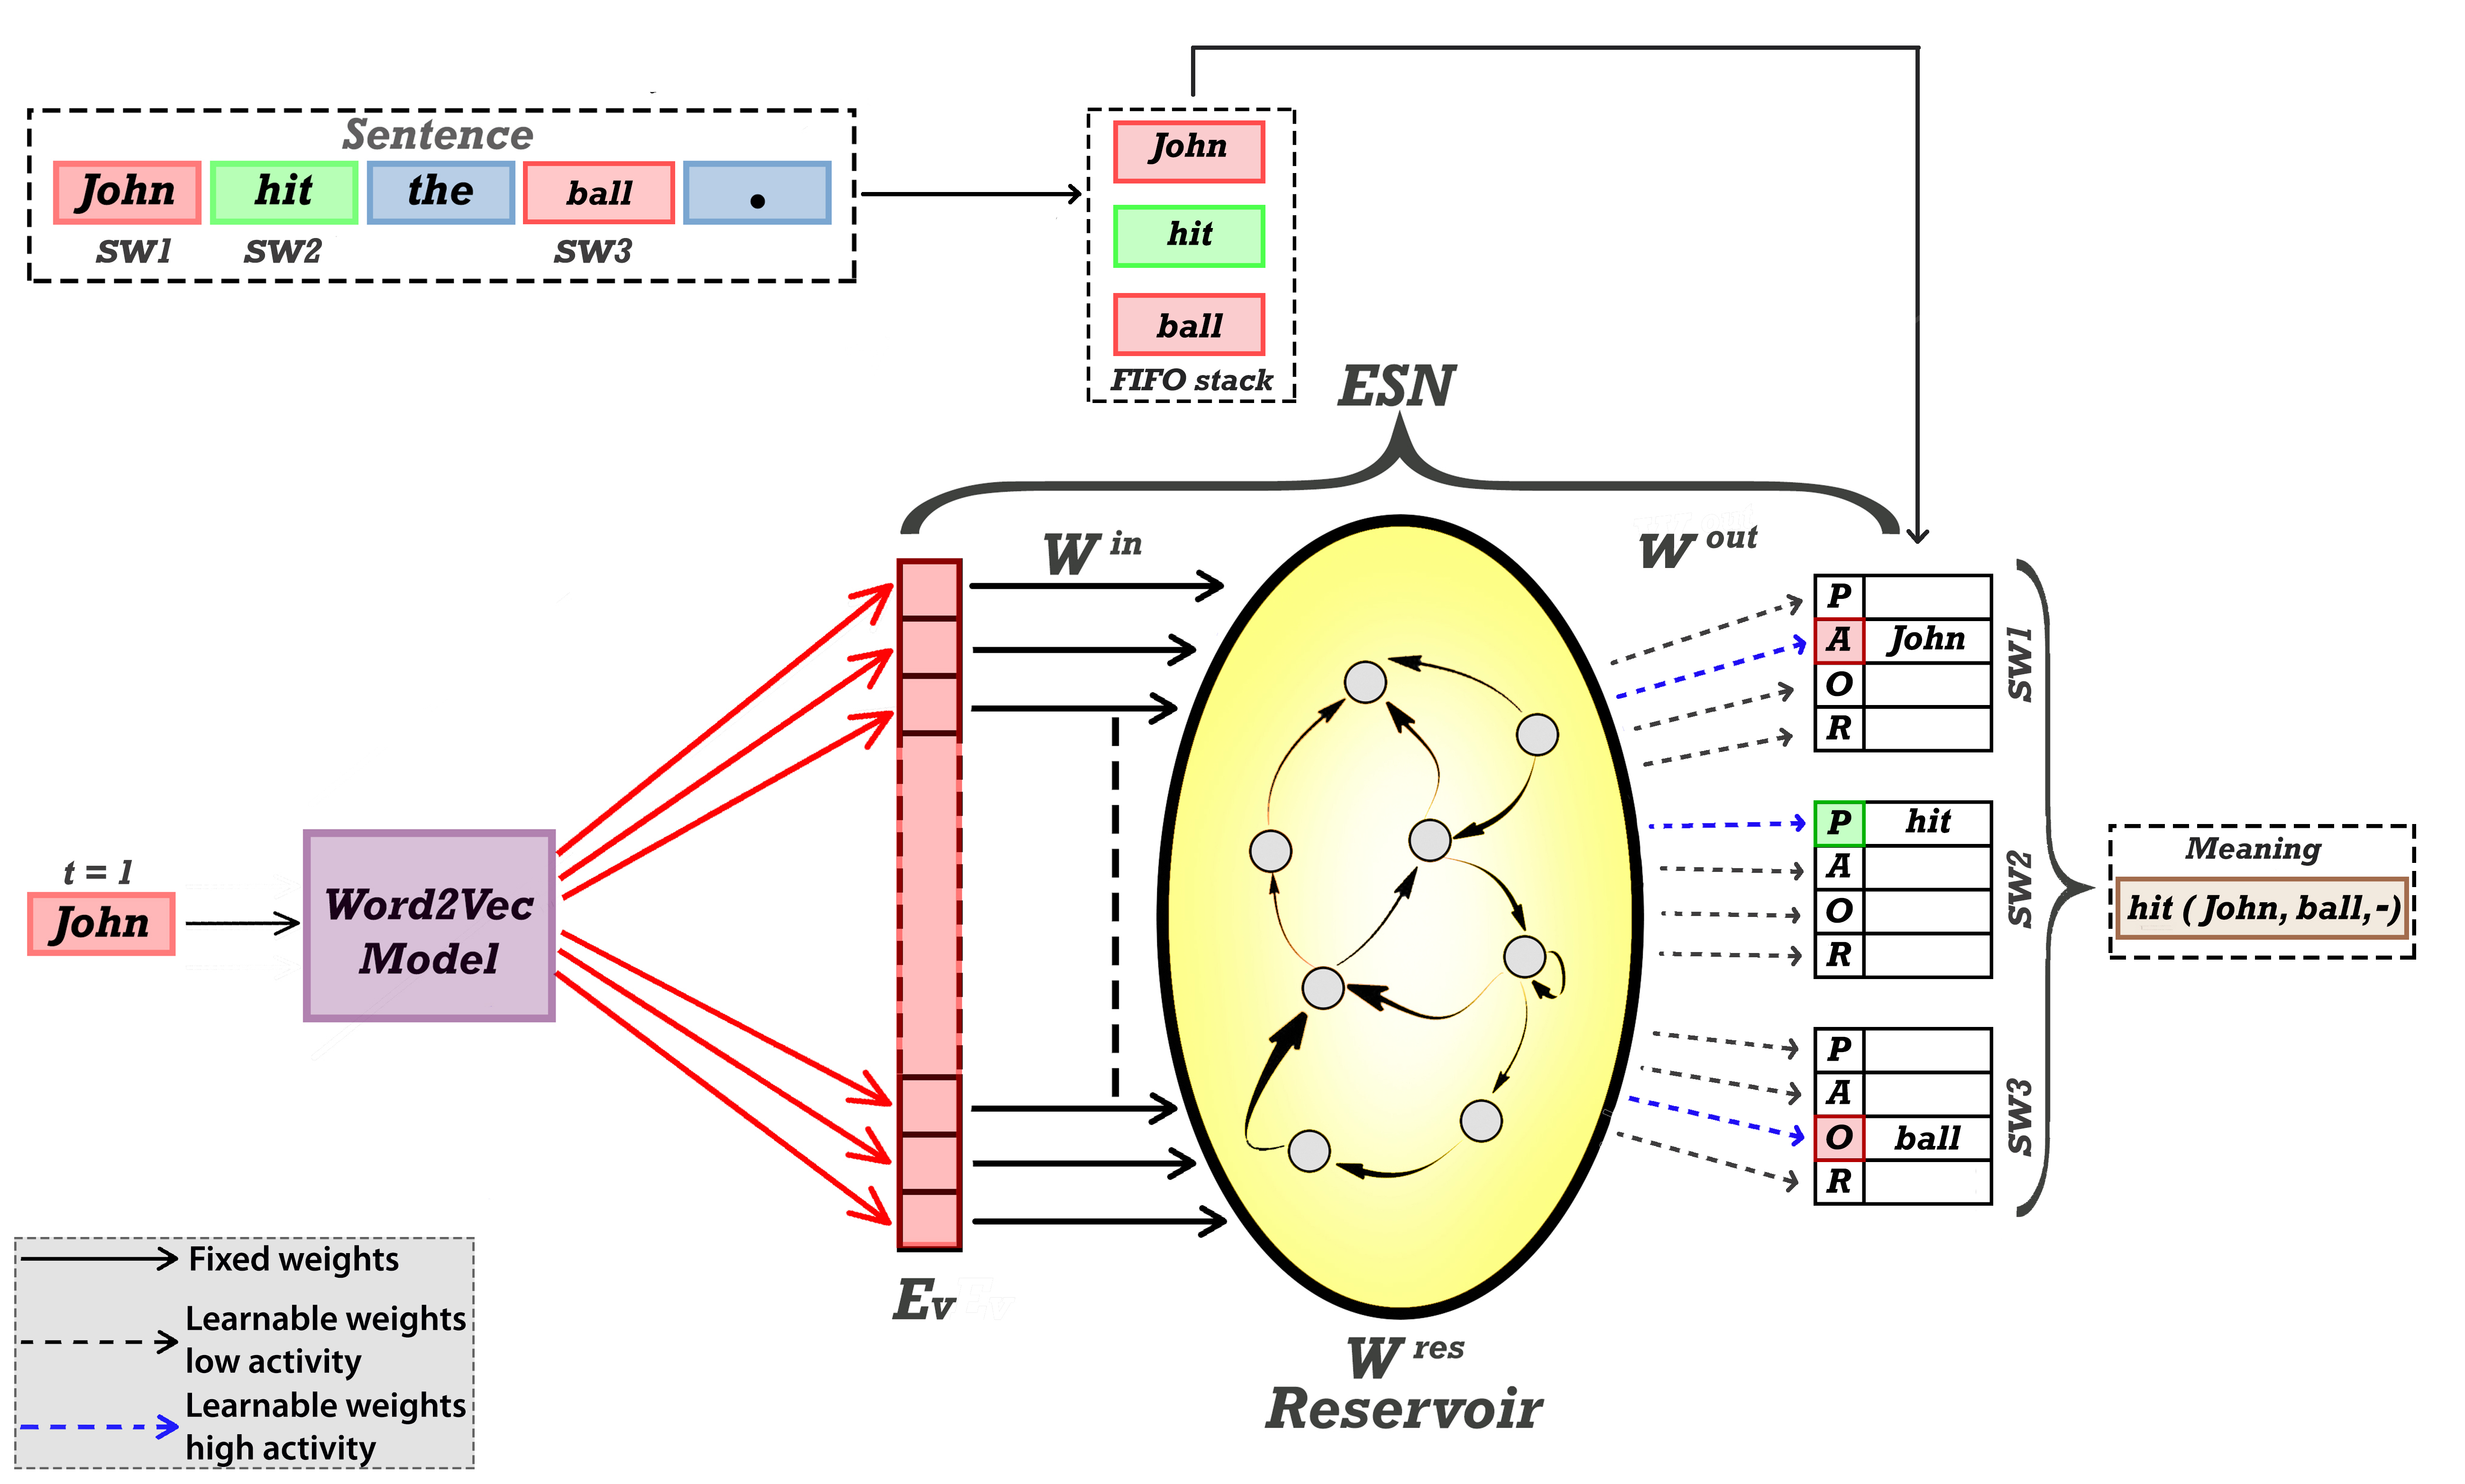
\includegraphics[width=0.9\linewidth]{w2v_esn_model}
\caption[Neural comprehension of the Word2Vec-$\theta$RARes model.]{\textbf{Word2Vec-$\theta$RARes language model:} {\small The figure shows the processing of a sentence at time step 1. Semantic words (specified in red and green respectively) are stored in a memory stack at the input. The word \textit{`John'} is input to Word2Vec model which generate a word vector of $E_{v}$ dimensions. The output word vector is then input to ESN for further processing. During training, the readout units are teacher-forced with the coded meaning of the input sentence (SW1: Agent, SW2: Predicate, SW3: Object). During testing, the readout units predict the coded meaning of input sentence. The meaning: hit(John, ball, -) is decoded from coded meaning by mapping the thematic roles with semantic words from memory stack. Adapted from \cite{xavier:2013:RT}}} 
\label{fig:model_variant_1}
\end{figure}

\begin{figure}[hbtp]
\centering
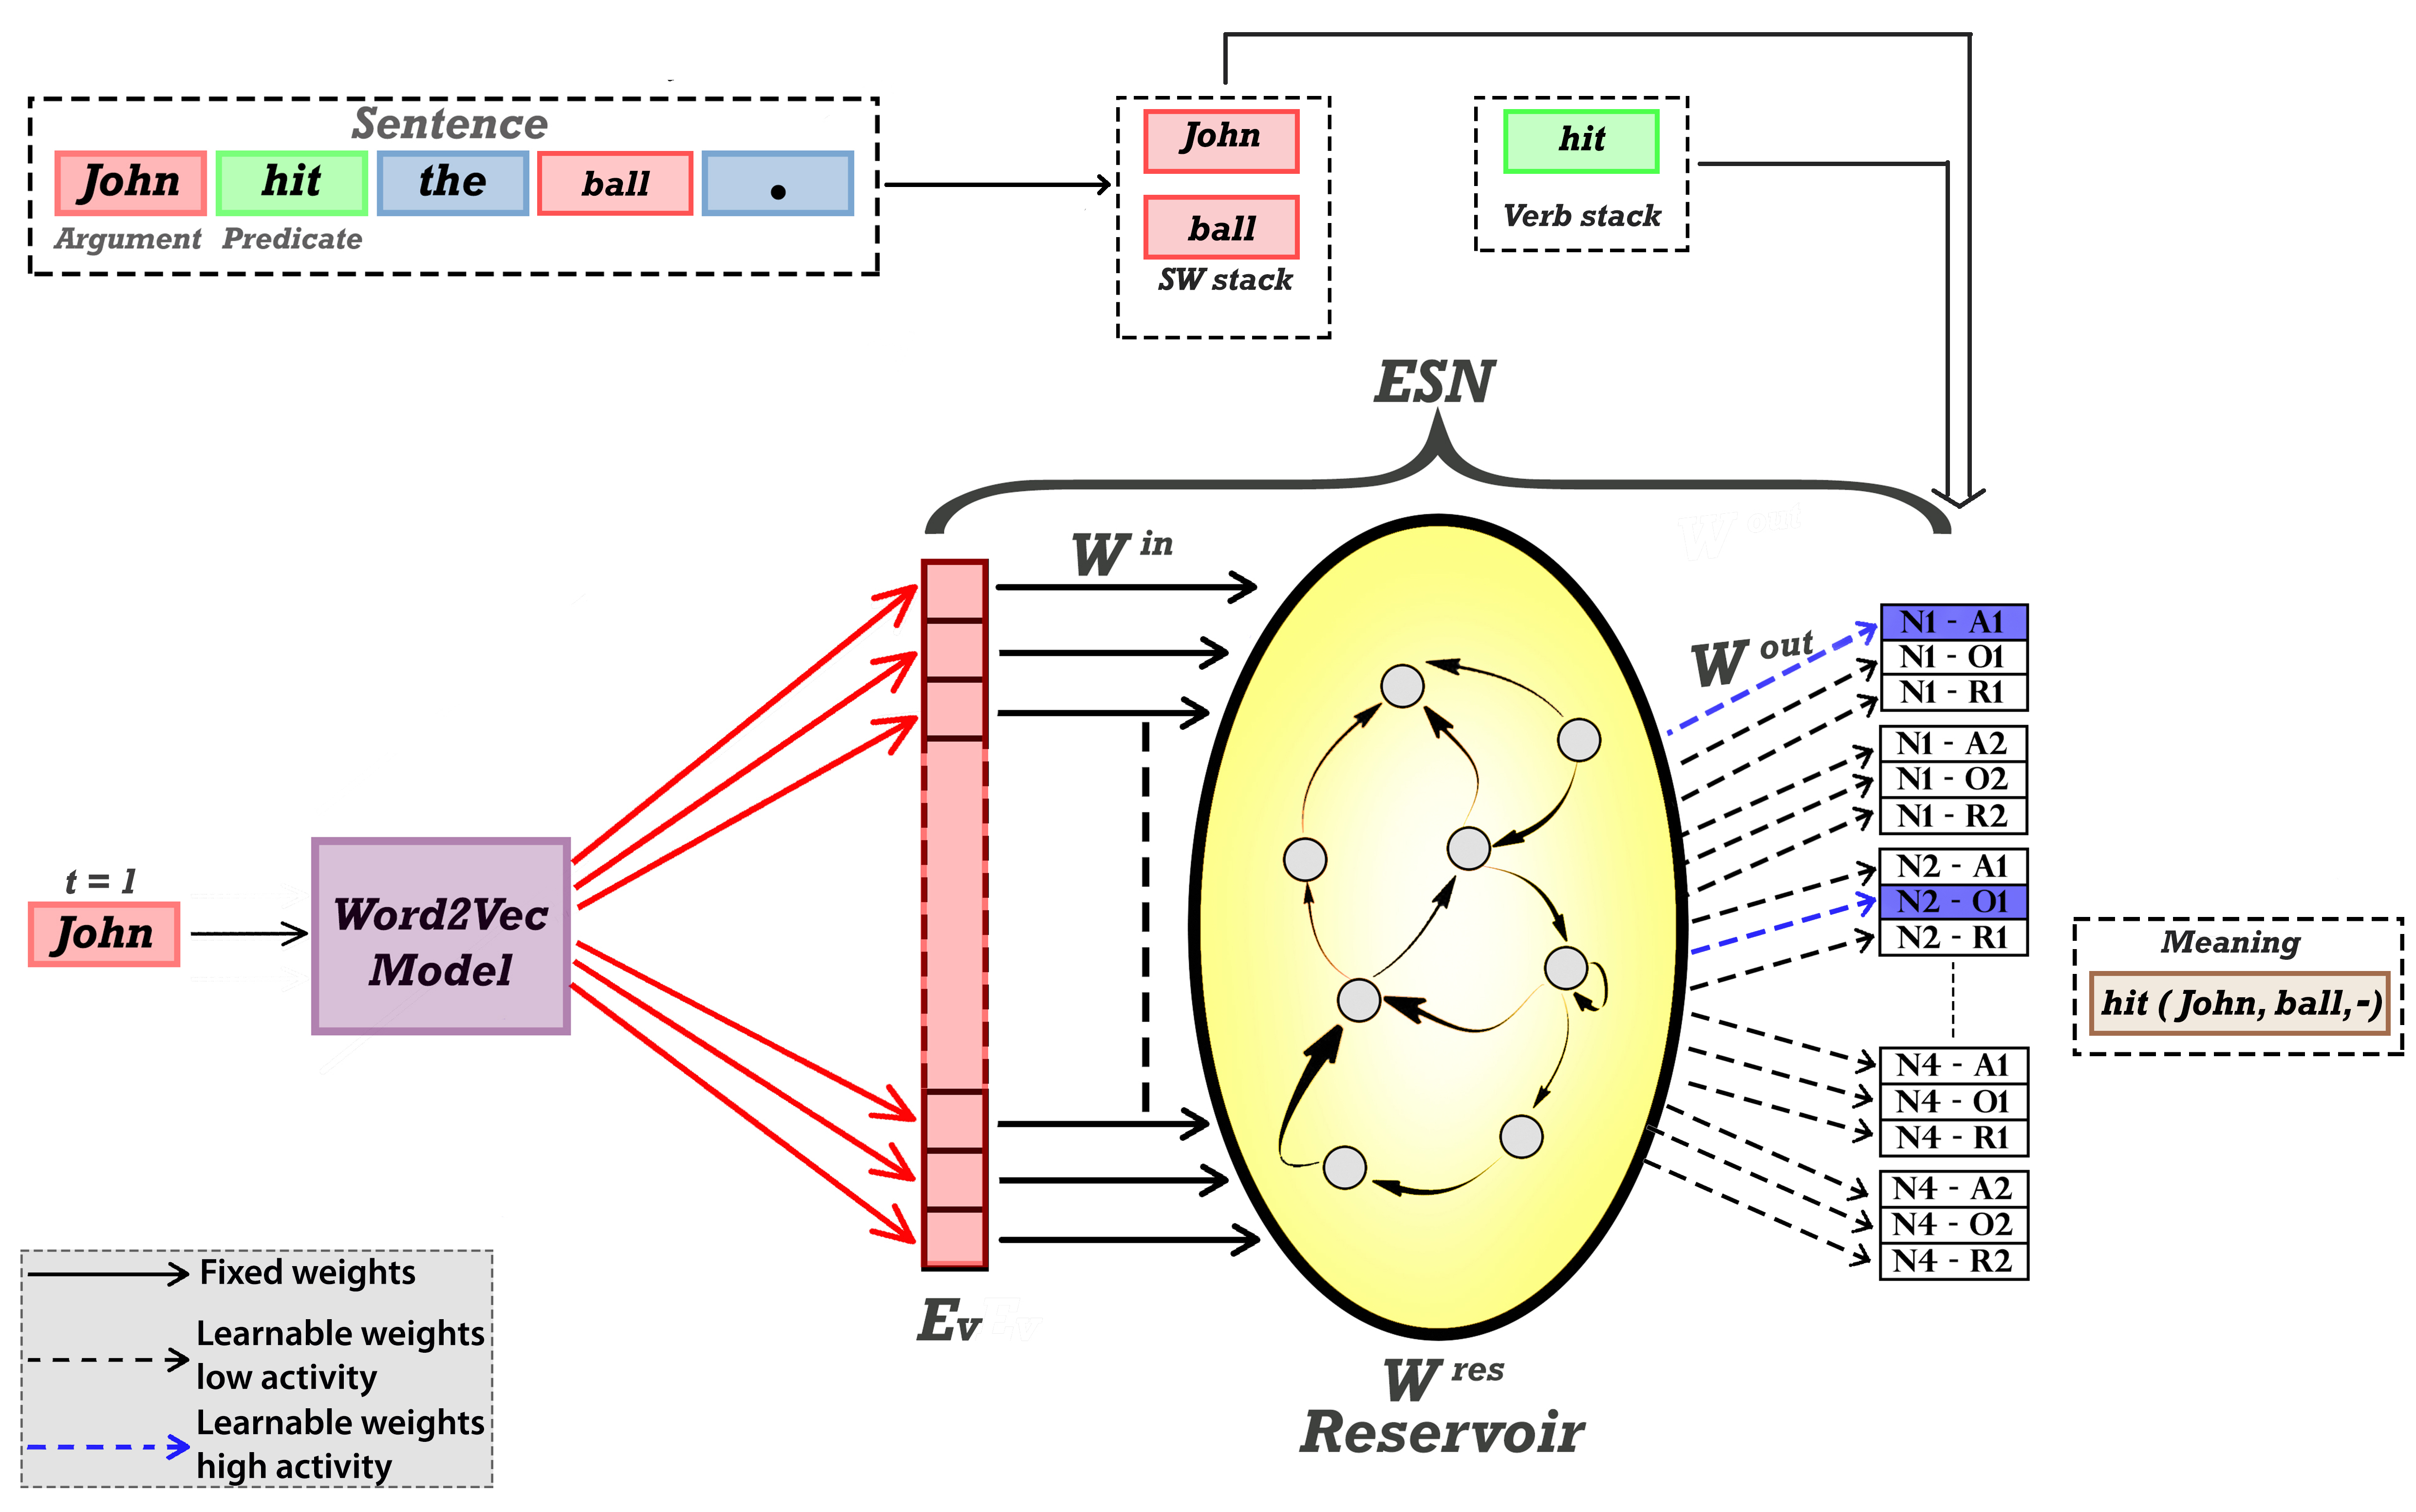
\includegraphics[width=0.9\linewidth]{w2v_esn_nv}
\caption[Neural comprehension of the Word2Vec-$\theta$RARes model with topologically modified coded meaning.]{\textbf{Word2Vec-$\theta$RARes Language model with topologically modified coded meaning:} {\small The figure shows the processing of a sentence with the topologically modified coded meaning at time step 1. Nouns and verbs (specified in red and green respectively) are stored in separate memory stack at the input. The word \textit{`John'} is input to Word2Vec model which generate a word vector of $E_{v}$ dimensions. The output vector is then input to ESN for further processing. During training, the readout units are teacher-forced with the coded meaning of input sentence (N1-A1, N2-O1). The output unit `N1-A1' represents that the first noun is an agent of the first verb in a sentence. During testing, the readout units predict the coded meaning of a semantic word with respect to a verb in an input sentence. The meaning ``hit(John, ball, -)" is decoded from coded meaning by mapping the thematic roles with semantic words from memory stacks. Adapted from \cite{xavier:2013:RT}}}
\label{fig:w2v_esn_nv}
\end{figure}

Figure \ref{fig:model_variant_1} shows the neural comprehension of the Word2Vec-$\theta$RARes model for thematic role assignment. Like $\theta$RARes model, a set of closed class words is created prior to training of the model. During the training, the sentences are presented to the model one at a time, word-by-word across time. Before presenting a sentence to the model, all the semantic words (not in closed class set) in the sentence are identified and placed in a FIFO memory stack (see fig. \ref{fig:model_variant_1}). This memory stack will be used later to decode the output coded meaning of the semantic words to the meaning of input sentence.

The size of the readout layer is $N_{sw} \times N_{tr} \times N_{verb}$: $N_{sw}$ and $N_{verb}$ are respectively the maximum number of semantic words and verbs any sentence can have in the corpus and $N_{tr}$ is the number of possible thematic role assignment for a semantic word. Thus each output neuron encodes the thematic role of a semantic word. In the figure \ref{fig:model_variant_1}, $N_{tr} = 4$ where the thematic roles Predicate, Agent, Object and Recipient are represented as P, A, O, R respectively. The model could also take the topologically modified but equivalent coded meaning of the sentences (see fig. \ref{fig:w2v_esn_nv}), where the role of each noun in a sentence is represented with respect to a verb \cite{xavier:2013:RT}. With the topologically modified coded meaning, the readout units contain $N_{noun} \times N_{verb}$ neurons where $N_{noun}$ is the maximum number of nouns any sentence can have in the corpus. 

The Word2Vec model receives the words from an input sentence over time and generates a word vector of $E_{v}$ dimension which is then used as an input to the ESN. The input layer of the ESN uses this word vector as input features for learning and predicting the thematic roles of the semantic words in the sentences. Thus the size of the input layer is same as the dimensionality of word vector i.e. $E_{v}$. During the training of the model, the readout layer of is also teacher-forced with the coded meaning of the input sentence. The output neurons have an activation of 1 if the corresponding thematic roles are present for the sentence, -1 otherwise. The output of the reservoir is accumulated for each time step during the presentation of a sentence. The accumulated reservoir states are then linearly combined with the readout activations (coded meaning of the input sentence) to learn the reservoir to readout ($W^{out}$) weights using the linear or ridge regression. The reservoir states of the ESN are reset before the presentation of the consequent sentences. The Word2Vec-$\theta$RARes model can be operated in two learning modes so that it learns to extract the coded meaning of the semantic words in the sentences:

\begin{enumerate}
\setlength{\itemsep}{\smallskipamount}

\item \textbf{Sentence Continuous Learning (SCL)}: In this learning mode, learning takes place from the beginning of the sentence. In other words, the coded meaning of the input sentence is made available to model from the onset of the first word of the sentence. Thus, the regression is applied from the onset of the first word in the sentence \cite{xavier:2013:RT}. \label{eg:SCL}

\item \textbf{Sentence Final Learning (SFL)}: In this mode, the learning takes places only at the end of the sentence \cite{xavier:2013:RT}. Hence, the teacher labels are only provided to the network at the end of sentence i.e. from the last word of the sentence. \label{eg:SFL}

\end{enumerate} 

\subsection{Decoding output}

As described earlier, the coded meaning of a sentence is defined as the description of thematic roles for all the semantic words in the sentence. The readout neurons of the model encode the thematic roles for all semantic words. Thus the output activations produced by the model while testing a sentence are thresholded at 0 for every semantic word. The maximum of all activation between $N_{tr}$ possible roles is taken as the coded meaning of a semantic word \cite{xavier:2013:RT}. A semantic word is said to have an incorrect coded meaning if the winning readout neuron is not the actual role of the semantic word. If there is no activation above the threshold for a semantic word, then this semantic word is considered to have no coded meaning \cite{xavier:2013:RT}. Combining the coded meaning of each semantic words forms the coded meaning of the sentence. The coded meaning of the sentence can then be mapped to the semantic words in FIFO memory stack to obtain the actual meaning of the sentence.
 
\subsection{Evaluation metrics}\label{sec:evaluation_metrics_1}

To evaluate the performance of the Word2Vec-$\theta$RARes language model, the same metrics that was used by Hianut et al. \cite{xavier:2013:RT} to evaluate the performance of the $\theta$RARes model was employed. The metrics compute the Meaning Error (ME) and the Sentence Error (SE). ME is the percentage of semantic words with incorrect coded meaning, whereas the SE is the percentage of sentences having at least one semantic word with incorrect coded meaning. Both the error measures are related, but there is no strict correlation between them \cite{xavier:2013:RT}. SE is a stricter measure than ME to evaluate model performance because a meaning error of $5\%$ cannot be used to estimate the sentence error, as this $5 \%$ incorrect words, can be from just one sentence or several sentences. 

Recall that if there are more than one action in a sentence, then each semantic word can have a possible role with respect to each action. Therefore, to evaluate the performance of the Word2Vec-$\theta$RARes model, not all the readout neurons are considered. For example, if a sentence has only three semantic words and two actions then only the readout neurons corresponding to these three semantic words with resepect to an action are analyzed, and the coded meaning of remaining neurons are ignored \cite{xavier:2013:RT}. 

\section{Word2Vec-ESN Classifier}\label{sec:model_variant}

\begin{figure}[hbtp]
\centering
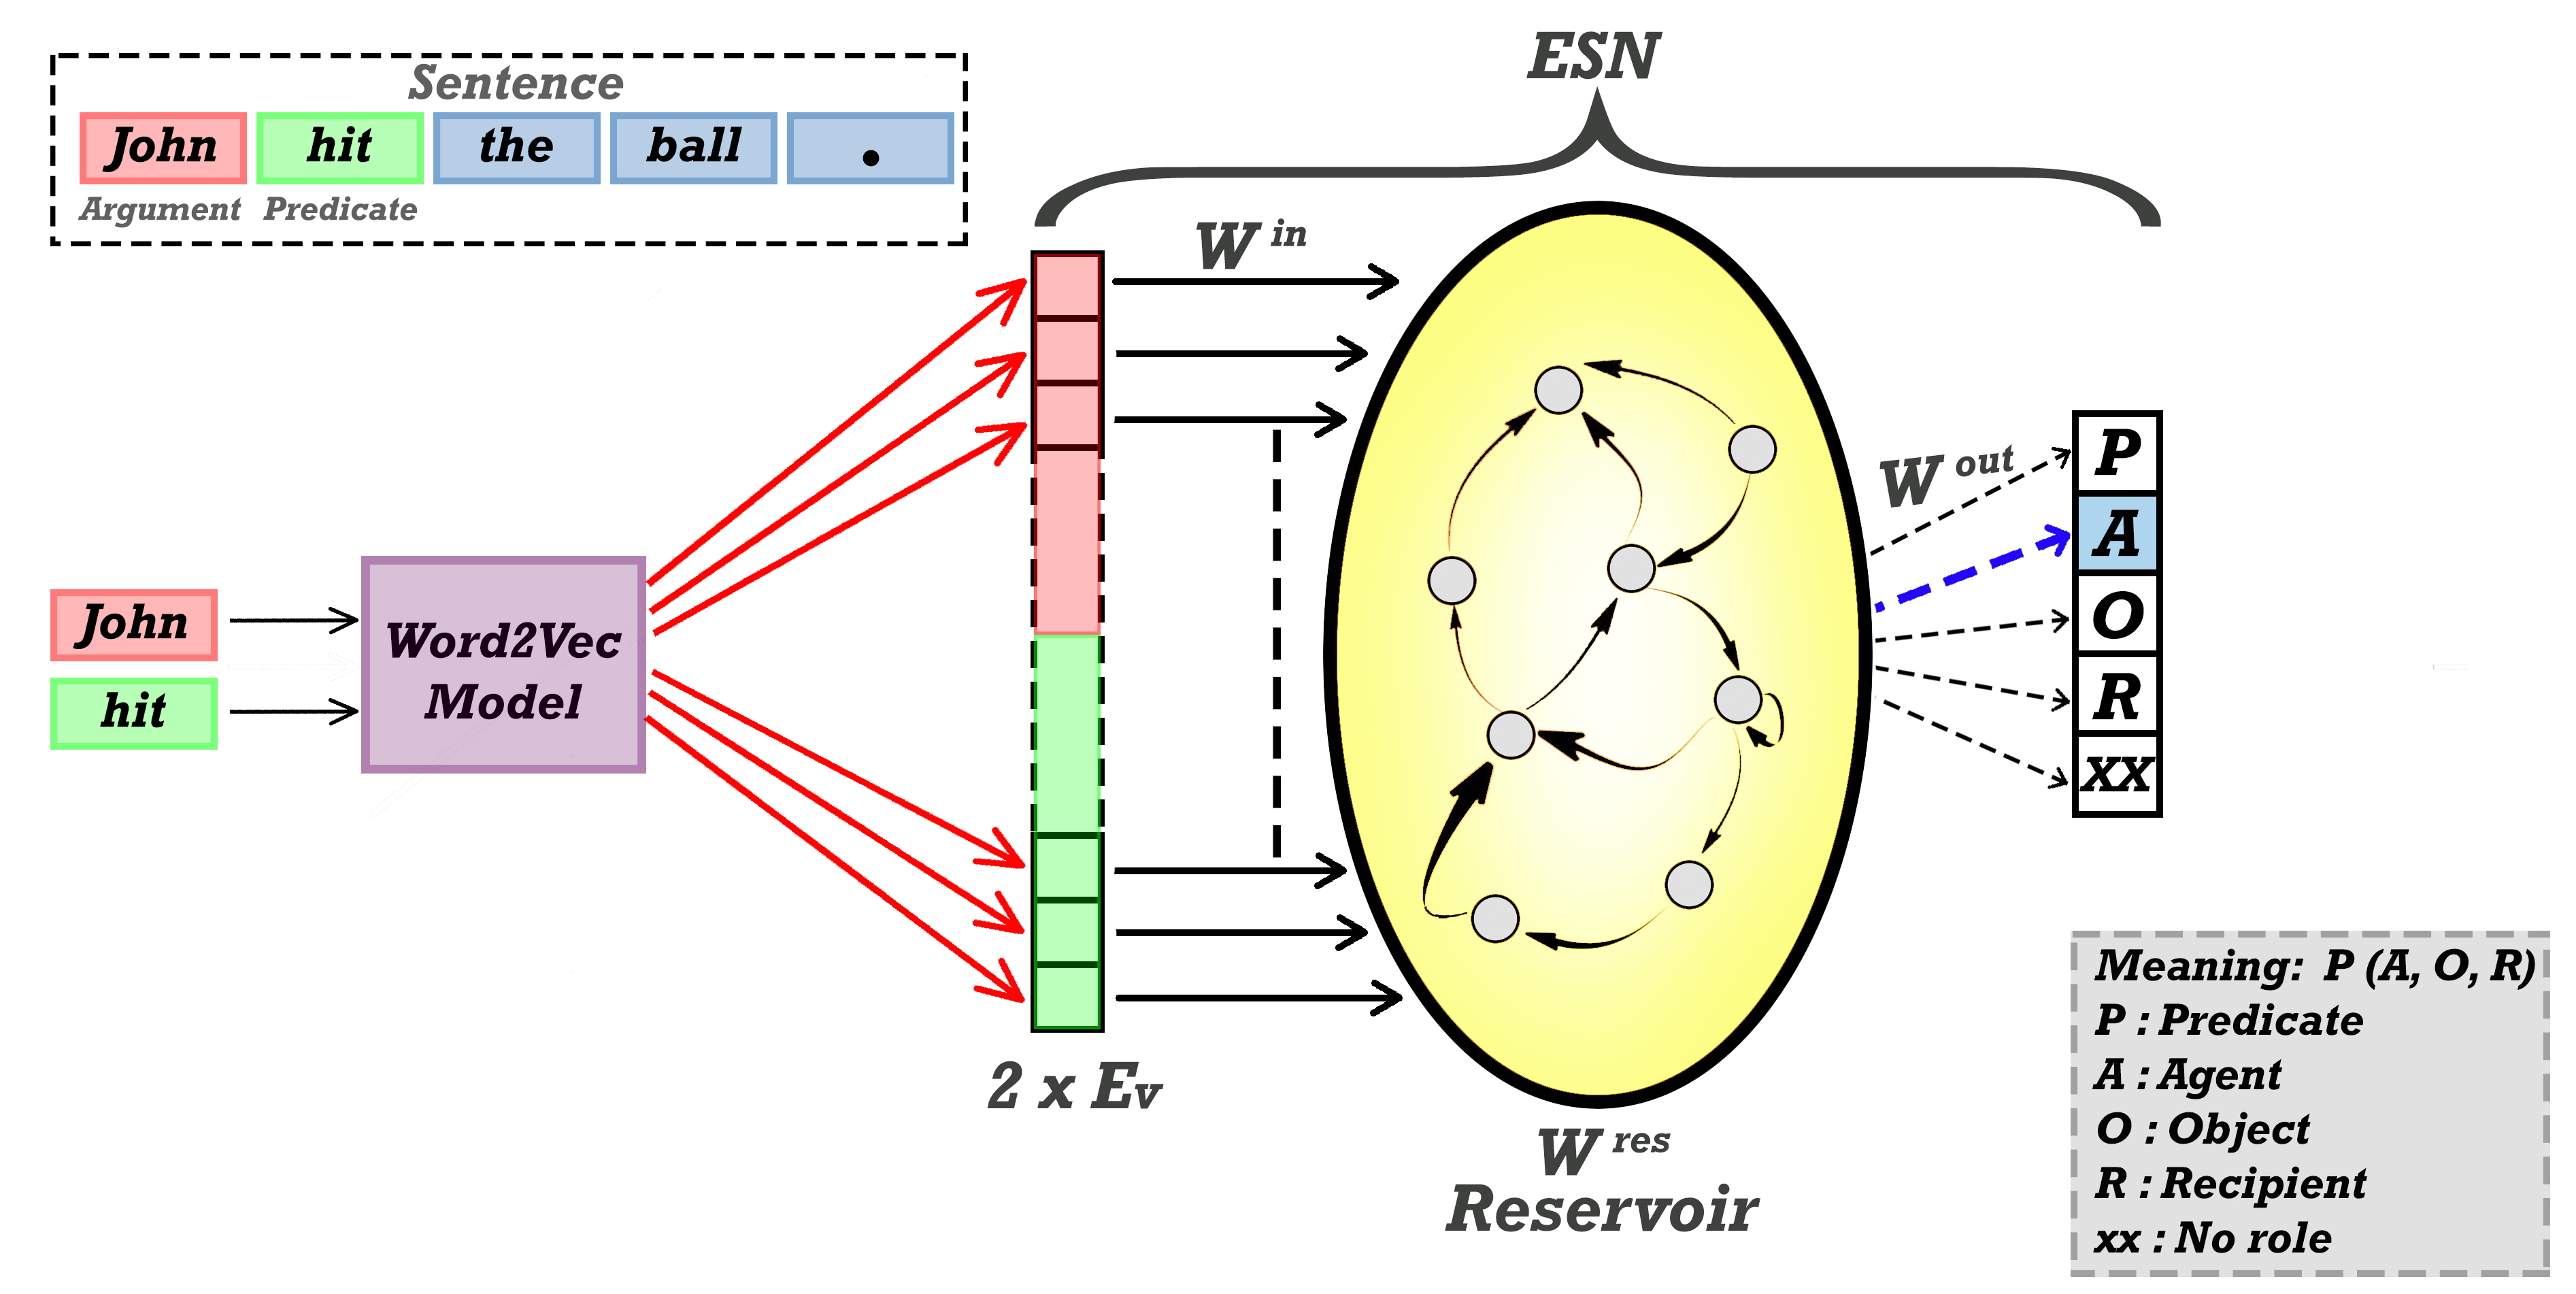
\includegraphics[width=1.0\linewidth]{w2v_esn_variant}
\caption[Functional organization of Word2Vec-ESN classifier for the TRA task.] {\textbf{Functional organization of Word2Vec-ESN classifier for the TRA task:} 
{\small At any instant of time, an argument-predicate pair (marked in red and green respectively) is input to the model. Word2Vec model generates a vector of $2 \times E_{v}$ dimensions. ESN takes the resultant vector for further processing. During the training, the readout neurons are presented with the role of input argument-predicate pair (e.g. `A' for Agent). The read-out weights ($W^{out}$, shown in dashed lines) are learned during the training. While testing, the readout unit predicts the role of argument-predicate pairs, which are then accumulated and decoded at the end of input sentence to form the meaning \textit{hit(John,ball,--)}. Inspired from \cite{end-to-end}
}}
\label{fig:model_variant_2}
\end{figure}


To ensure the objectivity of our findings, apart from the Word2Vec-ESN model, this research work also proposes a Word2Vec-ESN classifier. The basic architecture (see fig. \ref{fig:model_arch}) and initialization of Word2Vec-ESN classifier remain same to Word2Vec-$\theta$RARes model. Figure \ref{fig:model_variant_2} illustrates the functional organization of the Word2Vec-ESN classifier for the TRA task. Although the  Word2Vec-ESN classifier is architecturally (see fig. \ref{fig:model_arch}) similar to the Word2Vec-$\theta$RARes model, but varies in training objective and the way the sentences are processed. It treats the TRA task as a classification problem. The training objective of Word2Vec-ESN classifier is to classify the words of input sentences to a role with respect to the verbs and maximize the classification scores (i.e., F1-score, Precision, and Recall - see section \ref{sec:evaluation_metrics_2}) for each role. The roles typically include Predicate (P), Agent (A), Object (O), Recipient (R) and No-role (XX). 

Two input features play a major role in the Word2Vec-ESN classifier: argument and predicate. An argument describes the current word being processed and the predicate describes the verb with respect to which an argument is processed \cite{end-to-end}. So, if there are $N_{v}$ verbs in a sentence, then the same sentence is processed $N_{v}$ times. Thus each argument-predicate pair takes a role in a sentence. For example in the following sentence there are two predicates namely \textit{`chased'} and \textit{`ate'}. Therefore, this sentence will be processed twice, and each argument will take a role with respect a predicate \cite{end-to-end}. 

\begin{table}[H]
\centering
\label{tab:argument-predicate}
\begin{tabular}{lccccccccc}
Arguments $\rightarrow$ & the & dog & that & chased & the & cat & ate & the & rat \\
Predicate(`chased')      & XX  & A   & XX   & P      & XX  & O   & XX  & XX  & XX  \\
Predicate(`ate')         & XX  & A   & XX   & XX     & XX  & XX  & P   & XX  & O  
\end{tabular}
\end{table}

\noindent It is worth noticing that the classifier takes in input, the predicate with respect to which an argument is processed. To retrieve the predicates from a sentence, the Word2Vec-ESN classifier has to depend on a syntactic parser or Part Of Speech (POS) tagger. This limits the classifier from being an end-to-end system for the TRA task.  

\subsection{Training Word2Vec-ESN classifier}

To train the Word2Vec-ESN classifier, training sentences are presented to the model sequentially. Figure \ref{fig:model_variant_2} shows the processing of an example sentence by Word2Vec-ESN classifier. An input sentence is processed as many time as there are verbs in a sentence, forming multiple sequences. Thus the classifier takes an argument-predicate pair across the time as an input. The readout layer has five neurons each coding for a role (P, A, O, R, XX). Thus during the training, the role of the input argument-predicate pair is also teacher-forced to the model. Output neurons have an activation 1 if an input argument-predicate pair has the corresponding role, -1 otherwise. The Word2Vec model initially receives an argument-predicate pair of the input sentence and generates the distributed embeddings for both the input words. The generated word embeddings are concatenated and then taken by ESN as an input. Thus the size of ESN input layer is $2 \times E_{v}$: the first $E_{v}$ neurons takes the vector representation of the argument and remaining $E_{v}$ neurons for the predicate. The reservoir internal states are collected for an input sequence over time. Reservoir-to-readout ($W^{out}$) weights are then learned by using the linear or ridge regression on collected reservoir states and the readout activations. 

\subsection{Decoding output}

Recall that the Word2Vec-ESN classifier processes a sentence as many times as there are verbs in the sentence. Thus while testing, the output activations of the model is used to predict the role for an argument-predicate pair. The role having the highest output activation is considered as the role of an argument-predicate pair \cite{survey_multi_class}. The roles for all the argument-predicate pairs are collected and the meaning of a sentence with respect to a verb can then be interpreted by filling up the tagged words in form ``P(A, O, R)". For example, in the sentence ``John hit the ball." as shown in figure \ref{fig:model_variant_2}, the roles for each word-verb pair is used to deduce the meaning of the sentence as ``hit(John, ball, --)".

\subsection{Evaluation metrics}\label{sec:evaluation_metrics_2}

To analyze the performance of this Word2Vec-ESN classifier on TRA task, the confusion matrix or contingency table \cite{confusion_martrix:1998} is used and the classification scores: Accuracy, Precision, Recall, and F1-Score, are calculated for all possible roles. Higher the classification scores the better. To get the classification score of the model, scores of individual roles are macro-averaged, to get single real numbered scores. The reason for choosing macro-average is that it gives equal weights to all the roles, addressing the role imbalance problem \cite{macro_average:2005}. The same evaluation metrics was also used for CoNLL-04 and CoNLL-05 semantic role labeling shared task \cite{conll:2004,conll:2005}.

\begin{table}[H]
\centering
\caption{Confusion matrix to evaluate the Word2Vec-ESN classifier on the TRA task.}
\label{tab:argument-predicate}
\begin{tabular}{l|l|c|c|c|c|c|}
\multicolumn{2}{c}{}  &\multicolumn{5}{c}{\textbf{Predicted Roles}}\\
\cline{3-7}
\multicolumn{2}{c|}{} & \textbf{A} & \textbf{O} & \textbf{R} & \textbf{P} & \textbf{XX}\\
\hhline{|~|*6-|}
\multirow{5}{*}{\textbf{True Roles}}
& \textbf{A}     & \cellcolor{gray!25}$TP_{A}$ & $E_{A-O}$ & $E_{A-R}$ & $E_{A-P}$ & $E_{A-XX}$ \\
\hhline{~|*6-}
& \textbf{O}     & $E_{O-A}$ &\cellcolor{gray!25} $TP_{O}$ & $E_{O-R}$ & $E_{O-P}$ & $E_{O-XX}$ \\
\hhline{~|*6-}
& \textbf{R}     & $E_{R-A}$ & $E_{R-0}$ & \cellcolor{gray!25}$TP_{R}$ & $E_{R-P}$ & $E_{R-XX}$ \\
\hhline{~|*6-}
& \textbf{P}     & $E_{P-A}$ & $E_{P-0}$ & $E_{P-R}$ & \cellcolor{gray!25}$TP_{P}$ & $E_{P-XX}$ \\
\hhline{~|*6-}
& \textbf{XX}     & $E_{XX-A}$ & $E_{XX-O}$ & $E_{XX-R}$ & $E_{XX-P}$ & \cellcolor{gray!25}$TP_{XX}$ \\
\hhline{~|*6-}
\end{tabular}
\end{table}

The confusion matrix describes the predictions made by the model. The rows of the matrix correspond to the actual roles and the columns correspond the predictions made by the model. The top left to bottom right diagonal elements of this matrix represents the number of words for which the predicted role is equal to the actual role. So, higher the value of diagonal elements the better. The non-diagonal elements of the matrix represent the number of words which are incorrectly labeled. 

Using the confusion matrix, accuracy can be calculated as the ratio of the number of correctly labeled words to the total number of words (equation \ref{eqn:accuracy}). This accuracy measure specifies how often the classifier is correct \cite{classification_scores:2009}. 

\begin{equation}\label{eqn:accuracy}
Accuracy = \frac{\text{number of words correctly labelled}}{\text{total number of words}}
\end{equation}
 
However, accuracy measure can be distorting (because of accuracy paradox), when the dataset has words with significant role imbalance as it gives high scores to the models which merely predict the most frequent class. Thus accuracy measure cannot be used alone to evaluate the performance of the model \cite{accuracy_paradox_1:2008, accuracy_paradox_2:2014}. So, additional performance measures such as Precision (P), Recall (R), and F1-score (F1) are required to evaluate the model. All these measures take a value between 0 and 1. 

\textit{Precision} is defined as the ratio of True positive (TP) to False Positive(FP) and True Positive (equation \ref{eqn:precision}). It is the measure of accuracy of a role provided that a specific role has been predicted \cite{classification_scores:2009}.

\begin{equation}\label{eqn:precision}
Precision = \frac{\text{True Positive}}{\text{True Positive + False Positive}}
\end{equation}

\noindent From the confusion matrix above, the precision for the role Agent($A$) is be calculated as:
\[Precision(A) = \frac{TP_{A}}{(TP_{A}+E_{O-A}+E_{R-A}+E_{P-A}+E_{XX-A})}\]

\noindent \textit{Recall} is defined as the ratio of True Positive to True Positive and False Negative. It measures how good the model is in labeling the correct roles. It is also called \textit{'Sensitivity'} or \textit{'True Positive Rate'}. \cite{classification_scores:2009}.

\begin{equation}\label{eqn:recall}
Recall = \frac{\text{True Positive}}{\text{True Positive + False Negative}}
\end{equation}

\noindent Recall for the role `A', from the above confusion matrix is calculate as:
\[Recall(A) = \frac{TP_{A}}{(TP_{A}+E_{A-O}+E_{A-R}+E_{A-P}+E_{A-XX})}\]

\noindent F1-Score or (F1) is the harmonic mean of precision and recall. In other words, it represents the balance between precision and recall. The F1-score measure takes the false positive and the false negative into consideration. This score is useful whenever there is a class imbalance in the dataset \cite{classification_scores:2009} and is calculated as:

\begin{equation}\label{eqn:precision}
F1 = 2\times \frac{\text{Precision} \times{Recall }}{\text{Precision + Recall}}
\end{equation}
